% Define the page style
\fancypagestyle{chapterstyle}{
   \fancyhead[L]{\nouppercase{\rightmark}}
   \fancyhead[R]{Projet de fin d'études 2023-2024}
   \fancyfoot[C]{\vspace{20pt}\thepage} % Adjust the vertical space here
   \setlength{\headheight}{20pt}
   \setlength{\footskip}{30pt} % Adjust the value as needed
}
    \chapter{Contexte Général}
    \pagestyle{chapterstyle}    





\newpage
\vspace{1cm}
% \section{Introduction}


%%%%%%%%%%%%%%%%%%%% SECTION 2 %%%%%%%%%%%%%%%%%%%%%%%

\section{Introduction}
Ce chapitre expose le contexte général du projet. Dans un premier temps, il
présente l’organisme d’accueil 4D Logiciels Maroc. Dans un deuxième temps, il décrit le contexte,
la problématique et les objectifs derrière la réalisation de ce projet. Dans
un troisième temps, il décrit la conduite du projet mettant en lumière la méthodologie
suivie et la planification à l’aide du diagramme de Gantt.
\section{Présentation de l’organisme d’accueil}
\subsection{Organisme d'accueil}

4D Logiciels, fondée en 1984 par Laurent Ribardière, est une entreprise pionnière dans
le domaine du développement d’applications professionnelles. Son objectif initial était de
simplifier la création d’applications pour les entreprises en utilisant une base de données
relationnelle entièrement graphique, une innovation favorisée par l’industrie logicielle.\cite{4d}
\newline

% En tant que l’un des premiers éditeurs de logiciels français, 
% 4D a étendu son rayonnement à l’échelle internationale, avec 
% une présence sur les cinq continents et des filiales
% dans cinq pays, y compris le Maroc
\begin{figure}[h]
    \centering
    
\includegraphics[scale=0.8]{Images/logo-4d.jpg} % Replace with the actual filename of the IBM logo image
    \caption{Logo 4D\cite{4d}}
    \label{fig:Logo4D}
\end{figure}


% \subsubsection{Fiche signalétique de 4D Logiciels}


% \begin{table}[h!]
%     \centering
%     \caption{Fiche signalétique de 4D Logiciels}
%     \begin{tabular}{|>{\raggedright\arraybackslash}m{6cm}|>{\raggedright\arraybackslash}m{6cm}|}
%     \hline
%     Création & 1984 \\ 
%     \hline
%     Forme juridique & Société à Responsabilité Limitée à Associé Unique \\ 
%     \hline
%     Secteur & Conseil et développement de logiciels. \\ 
%     \hline
%     Siège social & Le Pecq, France \\ 
%     \hline
%     Taille de l’entreprise & 200-500 employés \\ 
%     \hline
%     \end{tabular}
%     \label{tab:fiche_signaletique}
% \end{table}

%%%%%%%%%%%%%%%%%%%% subsection 1 %%%%%%%%%%%%%%%%%%%%%%%

% \subsubsection{Histoire de 4D}
% En 1985, 4D a introduit le tout premier système de gestion
% de base de données relationnelles graphiques, offrant ainsi aux entreprises une nouvelle
% approche visuelle de la gestion des données. Deux ans plus tard, 4D a franchi une nouvelle
% étape en lançant le premier système de gestion de base de données 32 bits, établissant
% ainsi de nouveaux standards de performance et de puissance. En parallèle, 4D a étendu
% sa présence en créant 4D Inc. dans la Silicon Valley en 1987, 4D Deutschland,
% GmbH en 1988, renforçant ainsi son engagement sur le marché international.


% \begin{figure}[h]
%     \centering
%     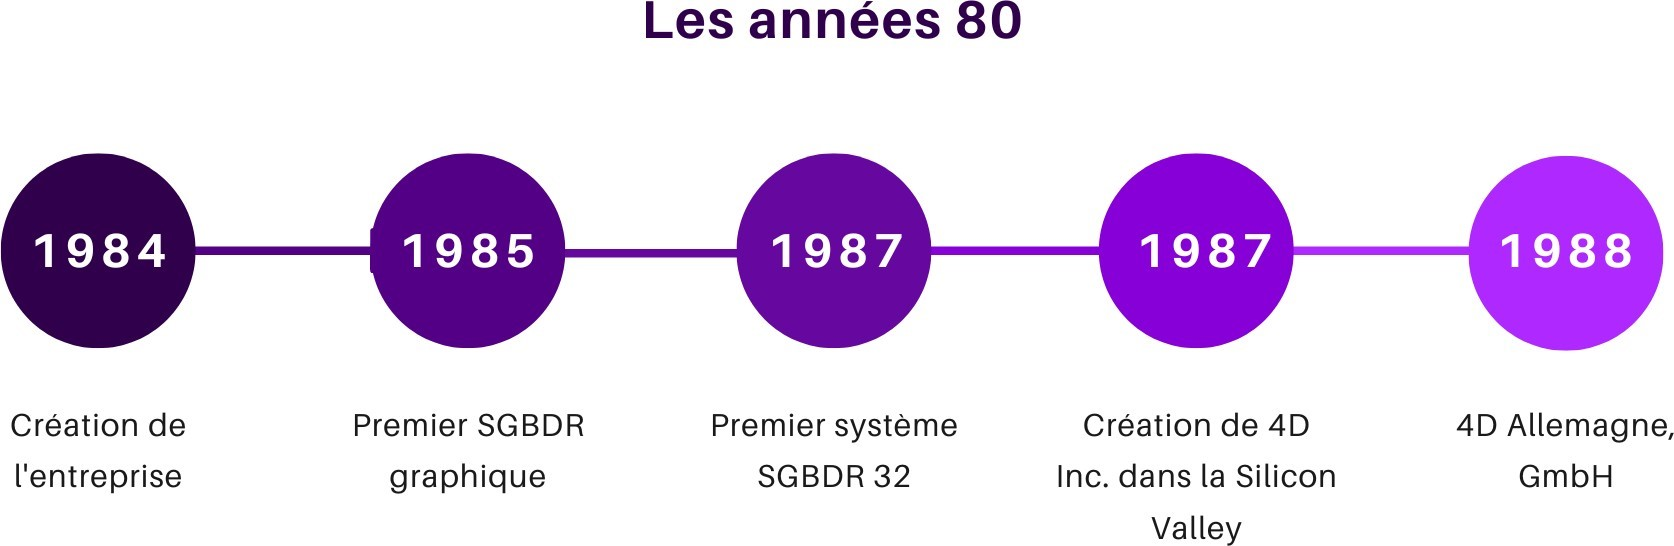
\includegraphics[scale=0.3]{Images/80.jpg} % Replace with the actual filename of the IBM logo image
%     \caption{4D dans les années 80}
%     \label{fig:Histoire80}
% \end{figure}
% \vspace{1cm}
% Dans les années 90, 4D a continué d’innover en lançant en 1992 le premier système
% de gestion de base de données Client/Serveur intégré. En 1995, 4D a introduit le premier
% système de gestion de base de données multiplateforme, permettant aux développeurs de
% créer des applications compatibles à la fois avec Mac et Windows en utilisant le même code
% source. En 1997, 4D a introduit le premier système de gestion de base de données Web
% dynamique, parallèlement, 4D a étendu sa présence mondiale en établissant 4D Japon en
% 1999, ce qui a renforcé par la suite son engagement sur le marché asiatique.
% \newline

% \begin{figure}[h]
%     \centering
%     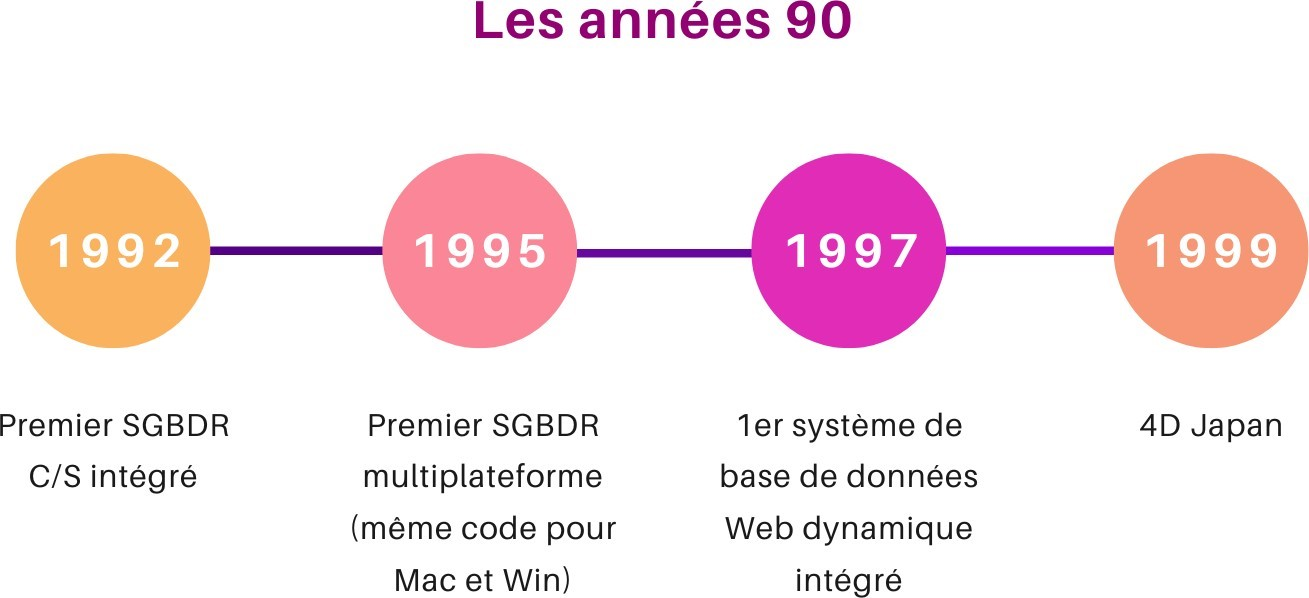
\includegraphics[scale=0.3]{Images/90.jpg} % Replace with the actual filename of the IBM logo image
%     \caption{4D dans les années 90}
%     \label{fig:Histoire90}
% \end{figure}
% % \vspace{lcm}

% Ensuite, 4D Australasie Pty Ltd a été fondée en 2002, consolidant ainsi sa présence
% en Australie et en Nouvelle-Zélande. En 2004, 4D a lancé la première IDE permettant de
% créer des applications Client/Serveur, Web ou SOA sans avoir à modifier le code source.
% En 2012, 4D a inventé la ligne de produits Wakanda, la première plateforme JavaScript de
% bout en bout. En parallèle, une autre filiale a été créée au Maroc en 2012 pour renforcer
% son existence sur le continent africain.
% En 2016, la ligne de produits Wakanda a été reconnue par Gartner en tant que ”Cool
% vendor”, confirmant ainsi l’engagement continu de 4D envers l’innovation et l’excellence
% dans le domaine des technologies de développement d’applications.
% \vspace{2cm}

% \begin{figure}[h]
%     \centering
%     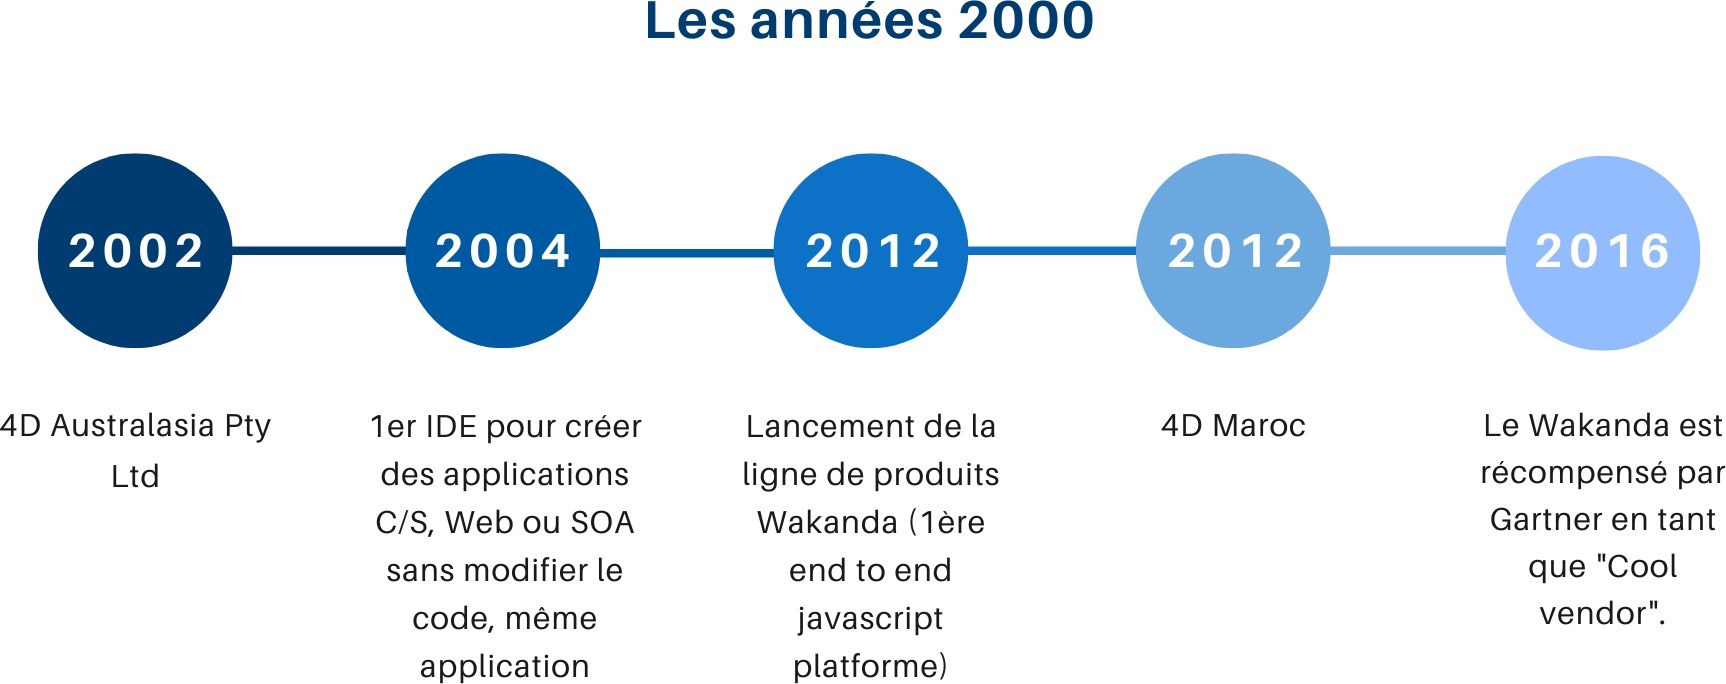
\includegraphics[scale=0.3]{Images/20.jpg} % Replace with the actual filename of the IBM logo image
%     \caption{4D dans les années 2000}
%     \label{fig:Histoire90}
% \end{figure}



% 4D v18 marque un véritable tournant dans l’histoire de 4D. 
% Cette version propose non seulement de multiples nouvelles 
% fonctionnalités mais aussi l’amélioration de fonctions existantes. 
% Elle introduit:
% \begin{itemize}
%     \item[•] \textbf{La gestion de version} pour changer la façon dont 
%     les équipes collaborent, le format texte des bases projets permet 
%     désormais de tirer pleinement parti des systèmes de gestion de 
%     version (par exemple, Git, SVN, etc.).
%     \item[•] \textbf{Une solution intégrée de chiffrement des données}, offrant en un seul clic une sécurité
%     maximum aux données des clients, basée sur l’un des algorithmes les plus sûrs, Advanced 
%     Encryption Standard (AES). 
%     \item[•] \textbf{ORDA (Object Relational Data Access)}, la technologie révolutionnaire d’accès et de présentation des 
%     données qui apporte de nouvelles fonctionnalités,
%     telles que le datastore distant, ouvrant de nouvelles perspectives 
%     et optimisant les performances du client/serveur. 
%     \item[•] \textbf{Le déploiment} facile des applications métiers sur des appareils mobiles avec 4D pour iOS. 
%     \item[•] \textbf{4D Write Pro}, un outil de PAO intégré à 4D, poursuit sa montée en puissance.
% \end{itemize}


%%%%%%%%%%%%%%%%%%%% subsection 2 %%%%%%%%%%%%%%%%%%%%%%%

\subsubsection{La structure du groupe 4D}
Le groupe 4D est composé d’un siège social situé en France, et de cinq filiales situées
aux États-Unis, en Allemagne, en Australie, au Japon, et au Maroc \cite{4d}.

% \vspace{lcm}
\begin{figure}[h]
    \centering
    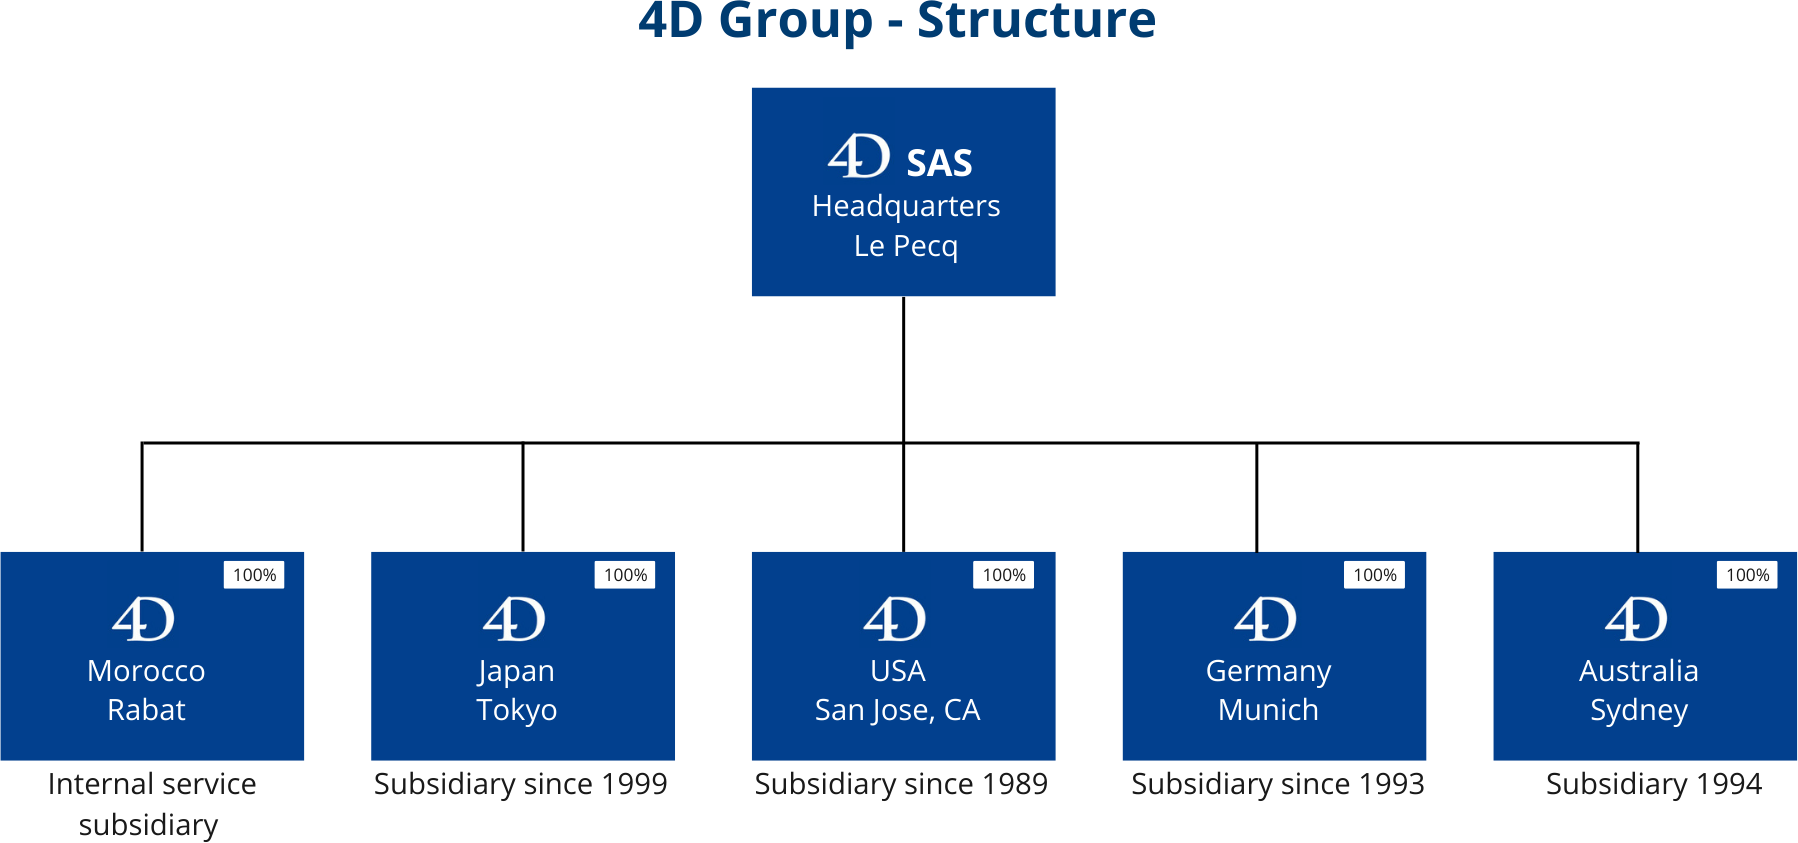
\includegraphics[scale=0.32]{Images/groupe.png} % Replace with the actual filename of the IBM logo image
    \caption{ La structure du groupe 4D\cite{4d}}
    \label{fig:groupe}
\end{figure}

% \subsubsection{Présence de 4D Logiciels dans le monde}
% Comme toute société renommée, 4D recourt à ses différents partenaires pour un rendu
% meilleur et un niveau d’expertise plus crédible. 4D connaît aussi une présence 
% internationale grâce à ses partenaires et ses distributeurs éparpillés dans le monde, 
% comme montre la figure suivante :


% \begin{figure}[h]
%     \centering
%     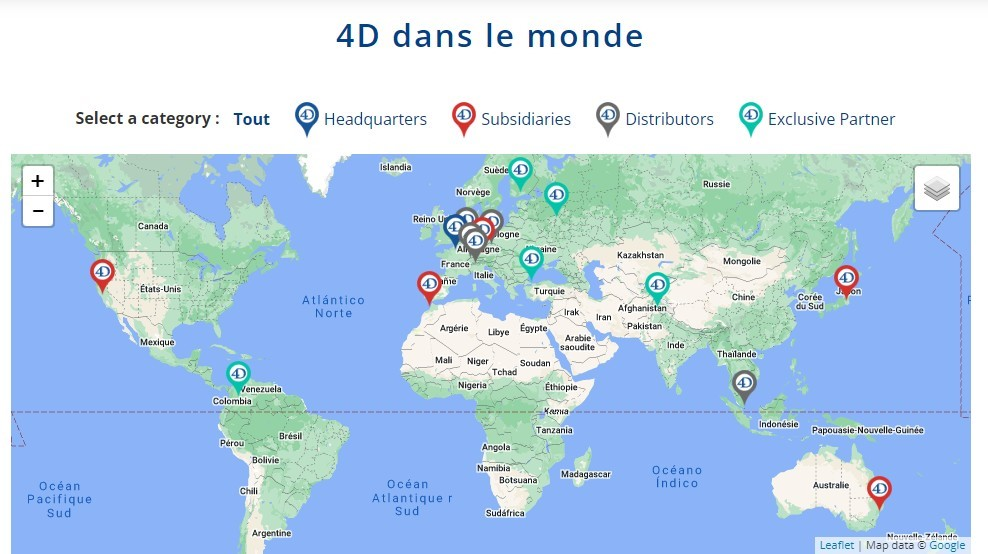
\includegraphics[scale=0.6]{Images/carte.jpg} % Replace with the actual filename of the IBM logo image
%     \caption{Présence de 4D Logiciels dans le monde}
%     \label{fig:carte}
% \end{figure}

% \vspace{3cm}

\subsubsection{Services offerts par 4D Logiciels}
4D Logiciels offre plusieurs services dans le domaine informatique, à savoir :
\begin{spacing}{1.1}
    
\begin{itemize}
    \item[ • ] \textbf{4D Professional Services: } Il offre une panoplie de services pour répondre aux besoins en développement logiciel, mettant à disposition une équipe qualifiée et des ressources de premier ordre à chaque étape du projet.
    \item[ • ] \textbf{Migration des bases de données 4D :} Il assure une transition sans heurts des bases de données 4D vers de nouveaux environnements ou versions, garantissant l’intégrité et la compatibilité des données tout en minimisant les perturbations opérationnelles.
    \item[ • ] \textbf{Migration 64-Bits : } Il assure une mise à niveau efficace des applications vers des environnements 64-bits, améliorant ainsi la performance, la stabilité et la sécurité des systèmes sans compromettre la fonctionnalité existante.
    \item[ • ] \textbf{Développement Mobile et Web :} Il fournit un accompagnement expert dans la conception et le développement sur mesure d’applications mobiles et web, en mettant un accent particulier sur l’optimisation de l’expérience utilisateur et l’intégration harmonieuse avec l’infrastructure informatique.
    \item[ • ] \textbf{Audit de sécurité :} Il réalise une évaluation approfondie de la sécurité des environnements informatiques, identifiant les vulnérabilités potentielles et proposant des stratégies proactives pour renforcer la protection des données et systèmes contre les menaces internes et externes.
    \item[ • ] \textbf{Service Assurance Qualité et Automatisation:} Il propose un service de tests automatisés, un service d’intégration continue ainsi qu’un service de tests fonctionnels et non fonctionnels dans l’optique d’améliorer l’efficacité des processus des applications métier de ces clients.
\end{itemize}
\end{spacing}


\subsubsection{Organigramme de l’organisme d’accueil}
La figure ci-dessous montre la hiéararchie de la direction générale de l’entreprise 4D
logiciels :

\begin{figure}[h]
    \centering
    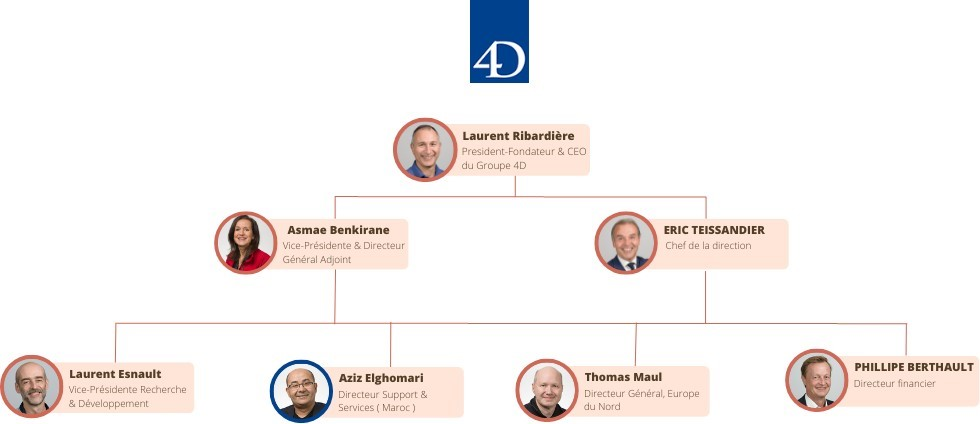
\includegraphics[scale=0.35]{Images/direction.jpg} % Replace with the actual filename of the IBM logo image
    \caption{La Direction Générale de 4D\cite{4d}}
    \label{fig:direction}
\end{figure}

\subsection{Plateforme 4D}
4D est une plateforme de développement productive qui permet aux clients de se concentrer 
sur leur modèle de données et les règles et spécificités de leur métier \cite{4d}. 
Elle prend en charge l’exécution native de leur code applicatif sous macOS et Windows. 
% Le Server 4D exécute leur applications simultanément sur les postes de travail, clients mobiles et sur le Web\cite{4d}. 
% Ils peuvent déployer des applications entièrement personnalisées sous leur propre marque.
\\
L'application 4D intègre :
\begin{spacing}{1.2}
    \begin{itemize}
        \item[•] une base de données graphique;
        \item[•] un compilateur;
        \item[•] un débogueur;
        \item[•] un système de sauvegarde et de réplication;
        \item[•] un serveur et client de services web.\\
    \end{itemize}    
\end{spacing}

Au sein de cette plateforme, nous pouvons utiliser que le langage 4D pour la programmation, 
ce dernier qui a évolué depuis son invention 
jusqu'à aujourd'hui avec la version V20.
Voici les anciennes versions de 4D dans la figure \ref{fig:versions}.
\begin{figure}[h]
    \centering
    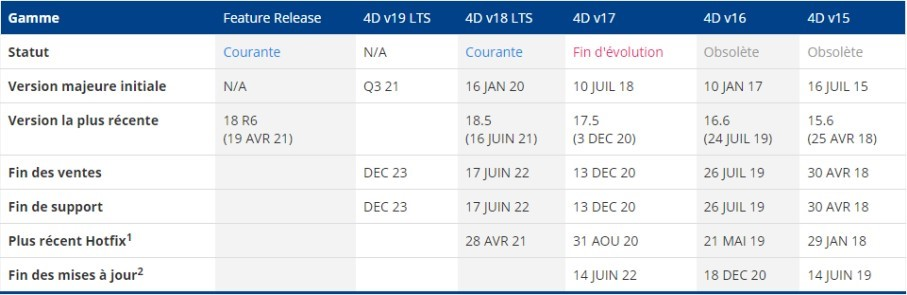
\includegraphics[scale=0.6]{Images/versions.jpg} % Replace with the actual filename of the IBM logo image
    \caption{Anciennes versions du langage 4D\cite{4d}}
    \label{fig:versions}
\end{figure}

% \subsection{Cadre du projet}
% Dans un environnement où la concurrence pour attirer les meilleurs talents
%  est de plus en plus intense, les entreprises doivent disposer d'outils 
%  efficaces pour gérer leur processus de recrutement. Actuellement, 
%  4D Logiciels utilise un système disparate et manuel pour le recrutement, 
%  ce qui entraîne des inefficacités et des pertes de temps. Cette situation 
%  rend difficile la gestion des candidatures, la traçabilité des étapes de 
%  recrutement, et la communication entre les recruteurs et les candidats.

% Afin de renforcer le niveau de ses collaborateurs, 4D Logiciels souhaite 
% simplifier et moderniser son processus de recrutement. L'objectif est de passer 
% d'un système essentiellement manuel à une solution plus intégrée et automatisée, 
% permettant d'améliorer l'efficacité, de réduire les délais de recrutement, 
% et d'offrir une meilleure expérience aux candidats.

% \subsection{Problématique}
% L'entreprise 4D Logiciels est confrontée à une gestion inefficace
%  de ses processus de recrutement, notamment lorsqu'elle publie 
%  des offres d'emploi et ouvre des opportunités de stage annuelles.
% 4D Logiciels reçoit un grand nombre de candidatures non triées,
% provenant de divers domaines, ce qui rend difficile la
% sélection des candidats les plus appropriés. Les méthodes 
% traditionnelles utilisées, telles que les emails, les tableurs 
% et les calendriers, ne permettent pas de gérer efficacement 
% ce flux de candidatures. De plus, les applications de recrutement
%  disponibles sur le marché ne répondent pas pleinement aux 
%  besoins spécifiques de l'entreprise en termes de processus 
%  de recrutement.

% En considérant les défis actuels du processus de recrutement chez
%  4D Logiciels, une interrogation primordiale se profile : 
%  comment transformer efficacement le processus de recrutement 
%  afin de surmonter les obstacles liés au traitement manuel des 
%  candidatures, à la dispersion des données et à la gestion 
%  disjointe des entretiens, assurant ainsi une sélection de 
%  candidats plus optimale et équitable pour l'organisation ?


% \subsection{Les objectifs}

% Pour répondre efficacement à la problématique identifiée,
% la solution proposée doit satisfaire les objectifs suivants :

% \begin{itemize}
%     \item Centraliser et Automatiser la Gestion des Candidatures
%     \item Améliorer la Sélection des Candidats 
%     \item Optimiser la Traçabilité et la Suivi des Étapes de Recrutement 
%     \item Faciliter la Communication et la Collaboration 
%     \item Analyser et Optimiser les Performances du Processus de Recrutement 
%     \item Offrir une Meilleure Expérience Candidat 
% \end{itemize}

% %%%%%%%%%%%%%%%%%%%% SECTION 4 %%%%%%%%%%%%%%%%%%%%%%%

\section{Présentation du projet}

\subsection{Cadre du projet }

% Actuellement, les processus de recrutement au sein de 4D Logiciels
% Maroc sont gérés de manière dispersée, chaque département utilise 
% sa propre méthode de recrutement. Cette fragmentation conduit à 
% des inefficacités et des difficultés de coordination. Le volume 
% élevé de candidatures et de CV reçus par mail ne peut pas être 
% traité de manière manuelle efficace, ce qui complique encore 
% davantage le suivi et la gestion des informations. En l'absence 
% d'un système centralisé, il devient impératif de moderniser et 
% de centraliser ces processus pour améliorer la cohérence et 
% l'efficacité de recrutement.
Le processus de recrutement chez 4D Logiciels Maroc repose beaucoup sur l'intervention des recruteurs, ce qui le rend lent et compliqué. 
Notamment, la réception des candidatures par mail nécessite des efforts considérables pour gérer chaque candidature et vérifier sa compatibilité 
avec l'offre proposée, surtout lorsque les offres publiées sont nombreuses.
\\
Pour bien comprendre la complexité de ce processus, nous allons illustrer cela avec des chiffres fournis par le département Professional 
Services (PS). Durant la période des Projets de Fin d'Études (PFE) 2024, ils ont reçu près de 200 CVs, ce qui a entraîné des retards dans 
le traitement des candidatures et des erreurs involontaires.
\\

En outre, les applications de recrutement disponibles, comme nous l'expliquerons dans la section \textbf{Benchmarking}, 
ne répondent pas aux besoins spécifiques de l'entreprise. Ainsi, il est primordial de moderniser et de centraliser ces processus pour améliorer 
la cohérence et l'efficacité du recrutement.


% Les processus de recrutement chez 4D Logiciels Maroc sont 
% actuellement fragmentés, chaque département utilise sa propre 
% méthode. Cette dispersion entraîne des inefficacités et des 
% difficultés de coordination, surtout avec le volume élevé de 
% candidatures et de CVs reçus par mail de divers domaines 
% (Par exemple, presque 200 CVs reçus par le département PS, Professional Services, uniquement 
% dans la pérode des PFE 2024), rendant  ainsi le traitement 
% manuel inefficace. De plus, l'utilisation d'emails et de 
% calendriers traditionnels complique beaucoup la sélection des candidats 
% appropriés. En outre, les applications de recrutement disponibles, comme le sera explicité dans la section du \textbf{Benchemarking}, 
% ne répondent pas aux besoins spécifiques de l'entreprise. Ainsi, 
% il est primordial de moderniser et de centraliser ces processus 
% pour améliorer le processus du recrutement.

\subsection{Problématique}
% L'entreprise 4D Logiciels est confrontée à une gestion inefficace
%  de ses processus de recrutement, notamment lorsqu'elle publie 
%  des offres d'emploi et ouvre des opportunités de stage annuelles.
% 4D Logiciels reçoit un grand nombre de candidatures non triées,
% provenant de divers domaines, ce qui rend difficile la
% sélection des candidats les plus appropriés. Les méthodes 
% traditionnelles utilisées, telles que les emails, les tableurs 
% et les calendriers, ne permettent pas de gérer efficacement 
% ce flux de candidatures. De plus, les applications de recrutement
%  disponibles sur le marché ne répondent pas pleinement aux 
%  besoins spécifiques de l'entreprise en termes de processus 
%  de recrutement.

En considérant les défis actuels du processus de recrutement chez
 4D Logiciels, une interrogation primordiale se profile : 
 comment transformer efficacement le processus de recrutement 
 afin de surmonter les obstacles liés au traitement manuel des 
 candidatures, à la dispersion des données et à la gestion 
 disjointe des entretiens, assurant ainsi une sélection de 
 candidats plus optimale et équitable pour l'organisme ?

\subsection{Objectifs}

% Pour répondre efficacement à la problématique identifiée,
% la solution proposée doit satisfaire les objectifs suivants :

% \begin{itemize}
%     \item[•] Centraliser et automatiser la gestion des candidatures
%     \item[•] Améliorer la sélection des candidats 
%     \item[•] Optimiser la traçabilité et le suivi des étapes de recrutement 
%     \item[•] Faciliter la Communication et la Collaboration 
%     \item[•] Analyser et optimiser les performances du processus de recrutement 
%     \item[•] Offrir une meilleure expérience candidat 
% \end{itemize}

% Les objectifs du projet sont :
% \begin{itemize}
%     \item[•] Centraliser les processus 
%     de recrutement en mettant en place une plateforme unique pour 
%     coordonner toutes les étapes.
%     \item[•] Automatiser le tri des candidatures en se basant sur les CVs.
%     \item[•] Réduire les inefficacités engendres par les processus actuels, 
%     en minimisant le temps de traitement des candidatures.
%     \item[•] Optimiser la sélection des candidats en facilitant 
%     l'identification des profils les plus qualifiés.
%     \item[•] Offrir une 
%     bonne expérience utilisateur grâce à une interface intuitive 
%     et professionnelle.
% \end{itemize}

Les objectifs du projet sont les suivants :
\begin{itemize}
    \item[•] Centraliser le processus de recrutement à travers une plateforme unique pour gérer toutes les étapes.
    % \item Automatiser le tri des candidatures en utilisant les CVs comme base de sélection.
    \item[•] Réduire les inefficacités des processus actuels en minimisant le temps de traitement des candidatures.
    \item[•] Optimiser la sélection des candidats en facilitant l'identification des profils les plus qualifiés.
    \item[•] Offrir une expérience utilisateur améliorée grâce à une interface intuitive et professionnelle.
\end{itemize}

\section{Conduite de projet}
\subsection{Méthodologie suivie}
% Pour mener à bien notre projet, nous avons adopté une approche itérative.
% Le projet a démarré avec un cahier des charges initial qui fournit une direction générale.
% Mais au fil du temps, nous avons pu le raffiner en faisant des reunions regulieres avec l'encadrant en entreprise
% Nous avons segmenté le travail en incréments, chaque itération se 
% concentre sur le développement de fonctionnalités spécifiques. 
% Des réunions régulières avec l'encadrant en entreprise, qui jouait le rôle de, ont permis de raffiner les besoins et de réévaluer 
% les priorités en fonction des retours obtenus.
Pour mener à bien notre projet, nous avons adopté une approche itérative, chaque itération se concentre sur le développement de 
fonctionnalités spécifiques. Certes, le projet a commencé avec un cahier des charges initial qui fournissait uniquement une direction 
générale, mais au fil du temps, nous l'avons affiné en organisant des réunions régulières avec notre encadrant en entreprise. Ces réunions 
ont également permis de réévaluer les priorités et les fonctionnalités en fonction des retours obtenus.

\subsection{Planification}
La mise en place de la planification a été réalisée à l’aide du logiciel de gestion de
projet GanttPRO, qui simplifie la planification et la mise en œuvre des projets grâce à
l’utilisation de diagrammes de Gantt qui fournit un aperçu sur le projet, y compris les
tâches, les dates, les délais, les dépendances.
% La figure ci-dessous montre la planification du projet, avec le diagramme de Gantt,
% qui s’étale sur une période de quatre mois, commençant par une formation globale sur
% le langage 4D et la plateforme 4D et l’analyse de l'ex, passant par la conception et le développement
% jusqu’aux tests end to end.

\begin{figure}[h]
    \centering
    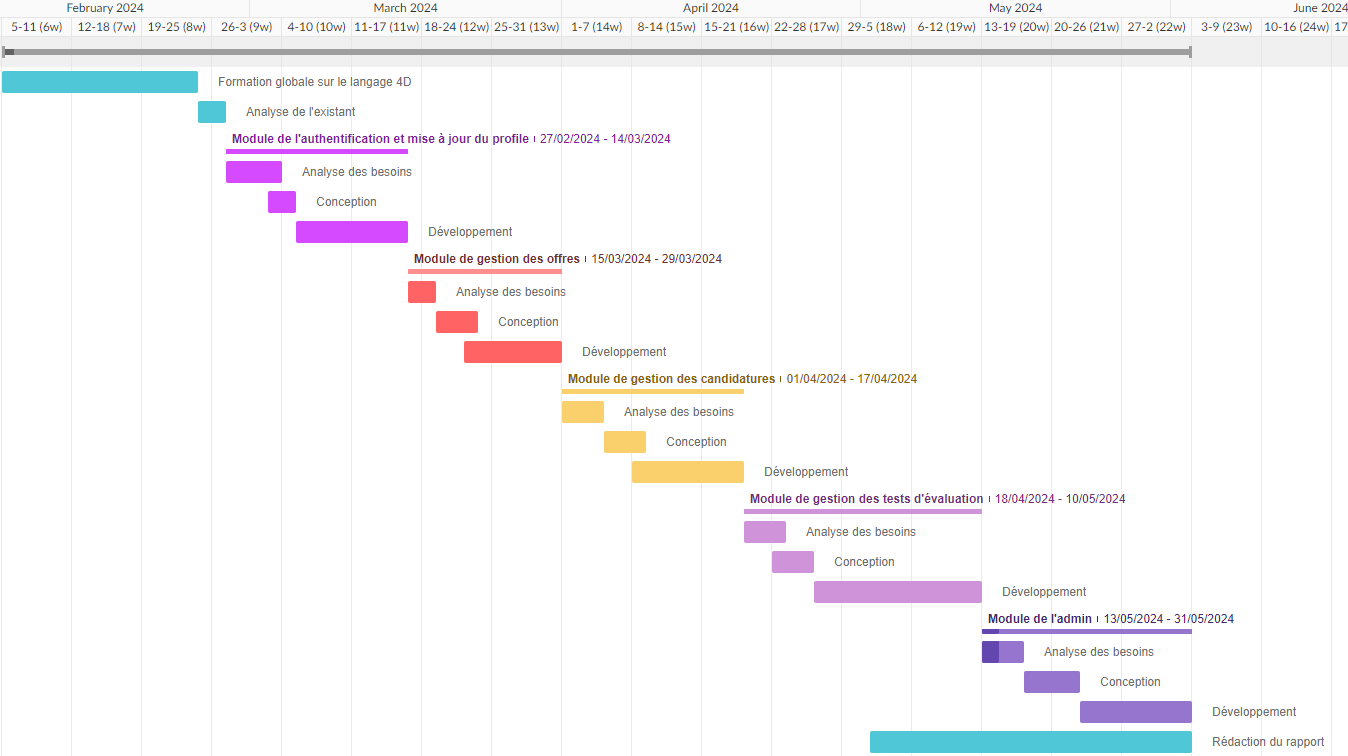
\includegraphics[scale=0.6]{diag/Gantt.png} % Replace with the actual filename of the IBM logo image
    \caption{Diagramme de Gantt}
    \label{fig:gantt}
\end{figure}

Pour mener à bien notre projet, une planification détaillée a été réalisée, comme illustré dans le diagramme de Gantt ci-dessous. 
La planification s'étend sur quatre mois et couvre plusieurs modules clés du système. En utilisant une approche itérative, le projet commence 
par une formation sur le langage 4D et une analyse de l'existant. Ensuite, les modules d'authentification et de mise à jour du profil, 
de gestion des offres, de gestion des candidatures, de gestion des tests d'évaluation, et de gestion administrative sont développés successivement, 
chacun passant par des cycles itératifs d'analyse des besoins, de conception, et de développement. La rédaction du rapport final clôture le projet, 
documentant les travaux effectués et les résultats obtenus.

\subsection{Outils de collaboration}
\subsubsection{Skype}
\begin{figure}[h]
    \centering
    
\includegraphics[scale=0.06]{Images/skype.png} % Replace with the actual filename of the IBM logo image
    \caption{Logo de Skype\cite{skype}}
    \label{fig:gantt}
\end{figure}

Skype est une plateforme de communication en ligne qui permet aux utilisateurs de communiquer par voix, par écrit et de partager des fichiers. 
Elle est couramment utilisée pour les appels vocaux, les appels vidéo et les réunions virtuelles. Nous avons utilisé Skype pour communiquer 
avec notre encadrant en entreprise, ce qui nous a permis de discuter de nos progrès, de nos difficultés et d'obtenir des conseils sur 
la résolution des problèmes. Skype a également facilité le partage de fichiers et de documents en temps réel, ce qui a grandement aidé notre 
collaboration.

\subsubsection{Git}
\begin{figure}[h]
    \centering
    
\includegraphics[scale=0.18]{Images/git.jpg} % Replace with the actual
    \caption{Logo de Git\cite{git}}
    \label{fig:git}
    \end{figure}
Git est un système de contrôle de version distribué qui permet aux développeurs de travailler
sur des projets en équipe. Il fournit une trace des modifications apportées au code
et permet de revenir à des versions précédentes en cas de besoin. Nous avons utilisé
Git pour gérer le code source du projet, ce qui nous a permis de travailler en
équipe et de partager nos modifications en temps réel. Git a également facilité
la gestion des conflits de versions et a permis de suivre l'évolution du projet

% \subsubsection{Gitlab}
% Gitlab est un outil de gestion de code source qui permet aux développeurs de gérer
% leurs projets en équipe. Il fournit des fonctionnalités telles que la gestion des tâches, 
% la gestion des versions et la gestion des dépôts
% Nous avons utilisé Gitlab pour gérer le code source du projet, ce qui nous a permis
% de travailler en équipe et de partager nos modifications en temps réel. Gitlab a
% aussi facilité la gestion des conflits de versions et a permis de suivre l'é
% volution du projet.

\subsubsection{Gitlab}

\begin{figure}[h]
    \centering
    
\includegraphics[scale=0.7]{Images/gitlab.jpg} % Replace with the actual
    \caption{Logo de GitLab\cite{gitlab}}
    \label{fig:gitlab}
\end{figure}


Gitlab est un outil de gestion de code source qui permet aux développeurs de collaborer sur leurs projets. Il offre des fonctionnalités telles que la gestion des tâches, des versions et des dépôts.

Nous avons utilisé Gitlab pour gérer le code source du projet, ce qui nous a permis de partager nos modifications en temps réel et de travailler efficacement en équipe. Gitlab a également facilité la gestion des conflits de versions et le suivi de l'évolution du projet.



Sur la figure \ref{fig:lab} est représenté notre code source dans GitLab.
    \begin{figure}[H]
        \centering
        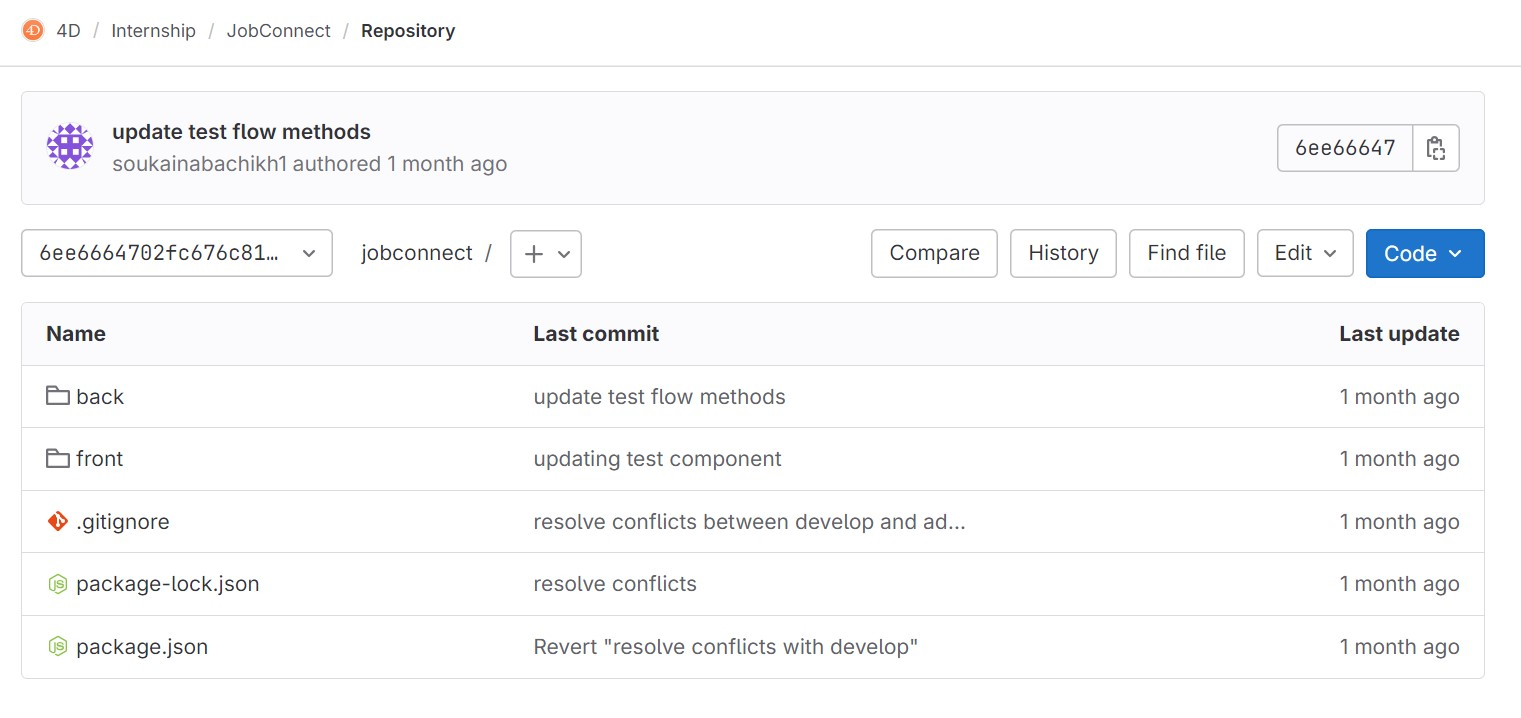
\includegraphics[scale=0.6]{gitlab/whole2.jpg} % Replace with the actual
        \caption{Aperçu global sur le projet dans GitLab}
        \label{fig:lab}
        \end{figure}
\section{Conclusion}
En guise de conclusion, ce chapitre a élucidé les fondements de l’étude du projet
menée; en fournissant une vue d’ensemble de l’organisme d’accueil, 4D Logiciels Maroc,
et de son fonctionnement interne. Il a également exposé le cadre du projet et la problématique à laquelle
il répond, mettant en lumière les défis auxquels l’entreprise est confrontée dans son
processus de recrutement actuel, ainsi que les objectifs à accomplir. Enfin, il a établi la
démarche et la planification du projet.


